% THIS DOCUMENT IS TAILORED TO REQUIREMENTS FOR SCIENTIFIC COMPUTING.  IT SHOULDN'T
% BE USED FOR NON-SCIENTIFIC COMPUTING PROJECTS
\documentclass[12pt]{article}

\usepackage{amsmath, mathtools}
\usepackage{amsfonts}
\usepackage{amssymb}
\usepackage{graphicx}
\usepackage{colortbl}
\usepackage{xr}
\usepackage{hyperref}
\usepackage{longtable}
\usepackage{xfrac}
\usepackage{tabularx}
\usepackage{float}
\usepackage{siunitx}
\usepackage{booktabs}
\usepackage{caption}
\usepackage{pdflscape}
\usepackage{afterpage}
\usepackage{adjustbox}
\usepackage{tikz}

\usepackage[round]{natbib}

%\usepackage{refcheck}

\hypersetup{
    bookmarks=true,         % show bookmarks bar?
      colorlinks=true,       % false: boxed links; true: colored links
    linkcolor=red,          % color of internal links (change box color with linkbordercolor)
    citecolor=green,        % color of links to bibliography
    filecolor=magenta,      % color of file links
    urlcolor=cyan           % color of external links
}

\input{../Comments.text}
\input{../Common.text}

% For easy change of table widths
\newcommand{\colZwidth}{1.0\textwidth}
\newcommand{\colAwidth}{0.13\textwidth}
\newcommand{\colBwidth}{0.82\textwidth}
\newcommand{\colCwidth}{0.1\textwidth}
\newcommand{\colDwidth}{0.05\textwidth}
\newcommand{\colEwidth}{0.8\textwidth}
\newcommand{\colFwidth}{0.17\textwidth}
\newcommand{\colGwidth}{0.5\textwidth}
\newcommand{\colHwidth}{0.28\textwidth}

% Used so that cross-references have a meaningful prefix
\newcounter{defnum} %Definition Number
\newcommand{\dthedefnum}{GD\thedefnum}
\newcommand{\dref}[1]{GD\ref{#1}}
\newcounter{datadefnum} %Datadefinition Number
\newcommand{\ddthedatadefnum}{DD\thedatadefnum}
\newcommand{\ddref}[1]{DD\ref{#1}}
\newcounter{theorynum} %Theory Number
\newcommand{\tthetheorynum}{TM\thetheorynum}
\newcommand{\tref}[1]{TM\ref{#1}}
\newcounter{tablenum} %Table Number
\newcommand{\tbthetablenum}{TB\thetablenum}
\newcommand{\tbref}[1]{TB\ref{#1}}
\newcounter{assumpnum} %Assumption Number
\newcommand{\atheassumpnum}{A\theassumpnum}
\newcommand{\aref}[1]{A\ref{#1}}
\newcounter{goalnum} %Goal Number
\newcommand{\gthegoalnum}{GS\thegoalnum}
\newcommand{\gsref}[1]{GS\ref{#1}}
\newcounter{instnum} %Instance Number
\newcommand{\itheinstnum}{IM\theinstnum}
\newcommand{\iref}[1]{IM\ref{#1}}
\newcounter{reqnum} %Requirement Number
\newcommand{\rthereqnum}{R\thereqnum}
\newcommand{\rref}[1]{R\ref{#1}}
\newcounter{nfrnum} %NFR Number
\newcommand{\rthenfrnum}{NFR\thenfrnum}
\newcommand{\nfrref}[1]{NFR\ref{#1}}
\newcounter{lcnum} %Likely change number
\newcommand{\lthelcnum}{LC\thelcnum}
\newcommand{\lcref}[1]{LC\ref{#1}}
\newcounter{ucnum} %Unlikely change number
\newcommand{\ucref}[1]{UC\ref{#1}}

\usepackage{fullpage}

\newcommand{\deftheory}[9][Not Applicable]
{
\newpage
\noindent \rule{\textwidth}{0.5mm}

\paragraph{RefName: } \textbf{#2} \phantomsection 
\label{#2}

\paragraph{Label:} #3

\noindent \rule{\textwidth}{0.5mm}

\paragraph{Equation:}

#4

\paragraph{Description:}

#5

\paragraph{Notes:}

#6

\paragraph{Source:}

#7

\paragraph{Ref.\ By:}

#8

\paragraph{Preconditions for \hyperref[#2]{#2}:}
\label{#2_precond}

#9

\paragraph{Derivation for \hyperref[#2]{#2}:}
\label{#2_deriv}

#1

\noindent \rule{\textwidth}{0.5mm}

}

\begin{document}

\title{Software Requirements Specification for \progname{}}
\author{Zhuo Zhang}
\date{January 23, 2026}

\maketitle

~\newpage

\pagenumbering{roman}

\tableofcontents

~\newpage

\section*{Revision History}

\begin{tabularx}{\textwidth}{p{3cm}p{2cm}X}
\toprule {\bf Date} & {\bf Version} & {\bf Notes}\\
\midrule
January 23, 2026 & 1.0 & Initial release\\
March 10, 2026 & 1.1 & Update from feedback\\
\bottomrule
\end{tabularx}



~\newpage

\section{Reference Material}

This section records information for easy reference.

\subsection{Table of Units}

Throughout this document SI (Syst\`{e}me International d'Unit\'{e}s) is employed
as the unit system. In addition to the basic units, several derived units are
used as described below. For each unit, the symbol is given followed by a
description of the unit and the SI name.
~\newline

\renewcommand{\arraystretch}{1.2}
\noindent \begin{tabular}{l l l}
  \toprule
  \textbf{symbol} & \textbf{unit} & \textbf{SI}\\
  \midrule
  \unit{\metre}   & length  & metre\\
  \unit{\kilogram}& mass    & kilogram\\
  \unit{\second}  & time    & second\\
  \unit{\ampere}  & electric current & ampere\\
  \unit{\coulomb} & electric charge & coulomb (C = \unit{\ampere\second})\\
  \unit{\newton}  & force   & newton (N = \unit{\kilogram\metre\per\second\squared})\\
  \unit{\joule}   & energy  & joule (J = \unit{\newton\metre})\\
  \unit{\tesla}   & magnetic flux density & tesla (T = \unit{\newton\per\ampere\metre})\\
  \unit{\volt}    & electric potential & volt (V = \unit{\joule\per\coulomb})\\
  \bottomrule
\end{tabular}

\subsection{Table of Symbols}

The table that follows summarizes the symbols used in this document along with
their units. The symbols are listed in alphabetical order.

\renewcommand{\arraystretch}{1.2}
\noindent \begin{longtable*}{l l p{12cm}} \toprule
\textbf{symbol} & \textbf{unit} & \textbf{description}\\
\midrule
$\mathbf{B}$ & \unit[per-mode=symbol]{\tesla} & magnetic flux density (magnetic field)\\
$\mathbf{E}$ & \unit[per-mode=symbol]{\newton\per\coulomb} & electric field\\
$\mathbf{F}$ & \unit[per-mode=symbol]{\newton} & force acting on the particle\\
$K$          & \unit[per-mode=symbol]{\joule} & kinetic energy of the particle\\
$L$          & \unit[per-mode=symbol]{\metre} & detector line location along the reference axis (e.g., $x=L$)\\
$m$          & \unit[per-mode=symbol]{\kilogram} & particle mass\\
$\mathbf{p}$ & \unit[per-mode=symbol]{\kilogram\metre\per\second} & linear momentum of the particle ($\mathbf{p}=m\mathbf{v}$)\\
$q$          & \unit[per-mode=symbol]{\coulomb} & particle charge\\
$r$          & \unit[per-mode=symbol]{\metre} & trajectory curvature radius (scenario-dependent)\\
$t$          & \unit[per-mode=symbol]{\second} & time\\
$a$          & \unit[per-mode=symbol]{\metre\per\second\squared} & acceleration\\
$t_{\text{hit}}$ & \unit[per-mode=symbol]{\second} & time at which the particle reaches the detector line\\
$\mathbf{v}$ & \unit[per-mode=symbol]{\metre\per\second} & particle velocity\\
$\mathbf{x}$ & \unit[per-mode=symbol]{\metre} & particle position\\
$\mathbf{x}_0$ & \unit[per-mode=symbol]{\metre} & initial position\\
$\mathbf{v}_0$ & \unit[per-mode=symbol]{\metre\per\second} & initial velocity\\
$\mathbf{x}_{\text{hit}}$ & \unit[per-mode=symbol]{\metre} & impact position on the detector line\\
\bottomrule
\end{longtable*}

\subsection{Abbreviations and Acronyms}

\renewcommand{\arraystretch}{1.2}
\begin{tabular}{l l}
  \toprule
  \textbf{symbol} & \textbf{description}\\
  \midrule
  A   & Assumption\\
  CLI & Command-Line Interface\\
  CSV & Comma-Separated Values\\
  DD  & Data Definition\\
  EM  & Electromagnetism\\
  GD  & General Definition\\
  GS  & Goal Statement\\
  IM  & Instance Model\\
  IVP & Initial Value Problem\\
  LC  & Likely Change\\
  ODE & Ordinary Differential Equation\\
  PS  & Physical System Description\\
  R   & Requirement\\
  SRS & Software Requirements Specification\\
  TM  & Theoretical Model\\
  \bottomrule
\end{tabular}\\

\subsection{Mathematical Notation}

\begin{itemize}
  \item Vectors are denoted in bold (e.g., $\mathbf{x}$, $\mathbf{v}$, $\mathbf{E}$, $\mathbf{B}$).
  \item A dot over a quantity denotes a time derivative, e.g., $\dot{\mathbf{x}} = d\mathbf{x}/dt$.
  \item The symbol $\times$ denotes the vector cross product.
  \item The notation $\|\mathbf{u}\|$ denotes the Euclidean norm (magnitude) of a vector $\mathbf{u}$.
  \item Subscript $0$ denotes an initial condition (e.g., $\mathbf{x}_0$, $\mathbf{v}_0$).
  \item Subscript \textit{hit} denotes the value at detector-plane impact (e.g., $\mathbf{x}_{\text{hit}}$, $t_{\text{hit}}$).
\end{itemize}

\newpage

\pagenumbering{arabic}

\section{Introduction}

Predicting the trajectory of a charged particle through piecewise-uniform
electromagnetic fields is a fundamental problem in accelerator and plasma physics.
Therefore, it is useful to have a program to simulate particle motion, model the
field-region-by-region deflection, and detect particle impacts on a detector line.
The document describes the program called \progname{}.

The following section provides an overview of the Software Requirements
Specification (SRS) for \progname{}.  This section explains the purpose of this
document, the scope of the requirements, the characteristics of the intended reader,
and the organization of the document.

\subsection{Purpose of Document}

The primary purpose of this document is to record the requirements of \progname{}.
Goals, assumptions, theoretical models, definitions, and other model derivation
information are specified, allowing the reader to fully understand and verify the
purpose and scientific basis of \progname{}.  With the exception of system
constraints, this SRS will remain abstract, describing what problem is being solved,
but not how to solve it.

This document will be used as a starting point for subsequent development phases,
including writing the design specification and the software verification and
validation plan.  The design document will show how the requirements are to be
realized, including decisions on the numerical algorithms and programming
environment.  The verification and validation plan will show the steps that will be
used to increase confidence in the software documentation and the implementation.
Although the SRS fits in a series of documents that follow the so-called waterfall
model, the actual development process is not constrained in any way.  Even when the
waterfall model is not followed, as Parnas and Clements point out
\cite{ParnasAndClements1986}, the most logical way to present the documentation is
still to ``fake'' a rational design process.

\subsection{Scope of Requirements}

The scope of the requirements includes the simulation of a single charged particle
under piecewise-uniform electromagnetic fields in two dimensions, and the detection
of the particle impact on a specified detector line.

\subsection{Characteristics of Intended Reader} \label{SecIntendedReader}

Reviewers of this documentation should have an understanding of
undergraduate-level physics (including classical mechanics and electromagnetism),
calculus, and ordinary differential equations.  The users of \progname{} can have
a lower level of expertise, as explained in Sec.~\ref{SecUserCharacteristics}.

\subsection{Organization of Document}

The organization of this document follows the template for an SRS for scientific
computing software proposed by \cite{SmithAndKoothoor2016}, \cite{SmithEtAl2007},
and \cite{SmithAndLai2005}.  The presentation follows the standard pattern of
presenting goals, theories, definitions, and assumptions.  For readers that would
like a more bottom-up approach, they can start reading the instance models and
trace back to find any additional information they require.

The goal statements are refined to the theoretical models and the theoretical
models to the instance models.

\section{General System Description}

This section provides general information about the system. It identifies the
interfaces between the system and its environment, describes the user
characteristics and lists the system constraints.

\subsection{System Context}

Figure~\ref{Fig_SystemContext} shows the system context. A circle represents an
entity external to the software, the user and the input/output files in this
case. A rectangle represents the software system itself (\progname{}). Arrows
are used to show the data flow between the system and its environment.

\begin{figure}[h!]
\begin{center}
 \IfFileExists{diagram.jpg}{%
  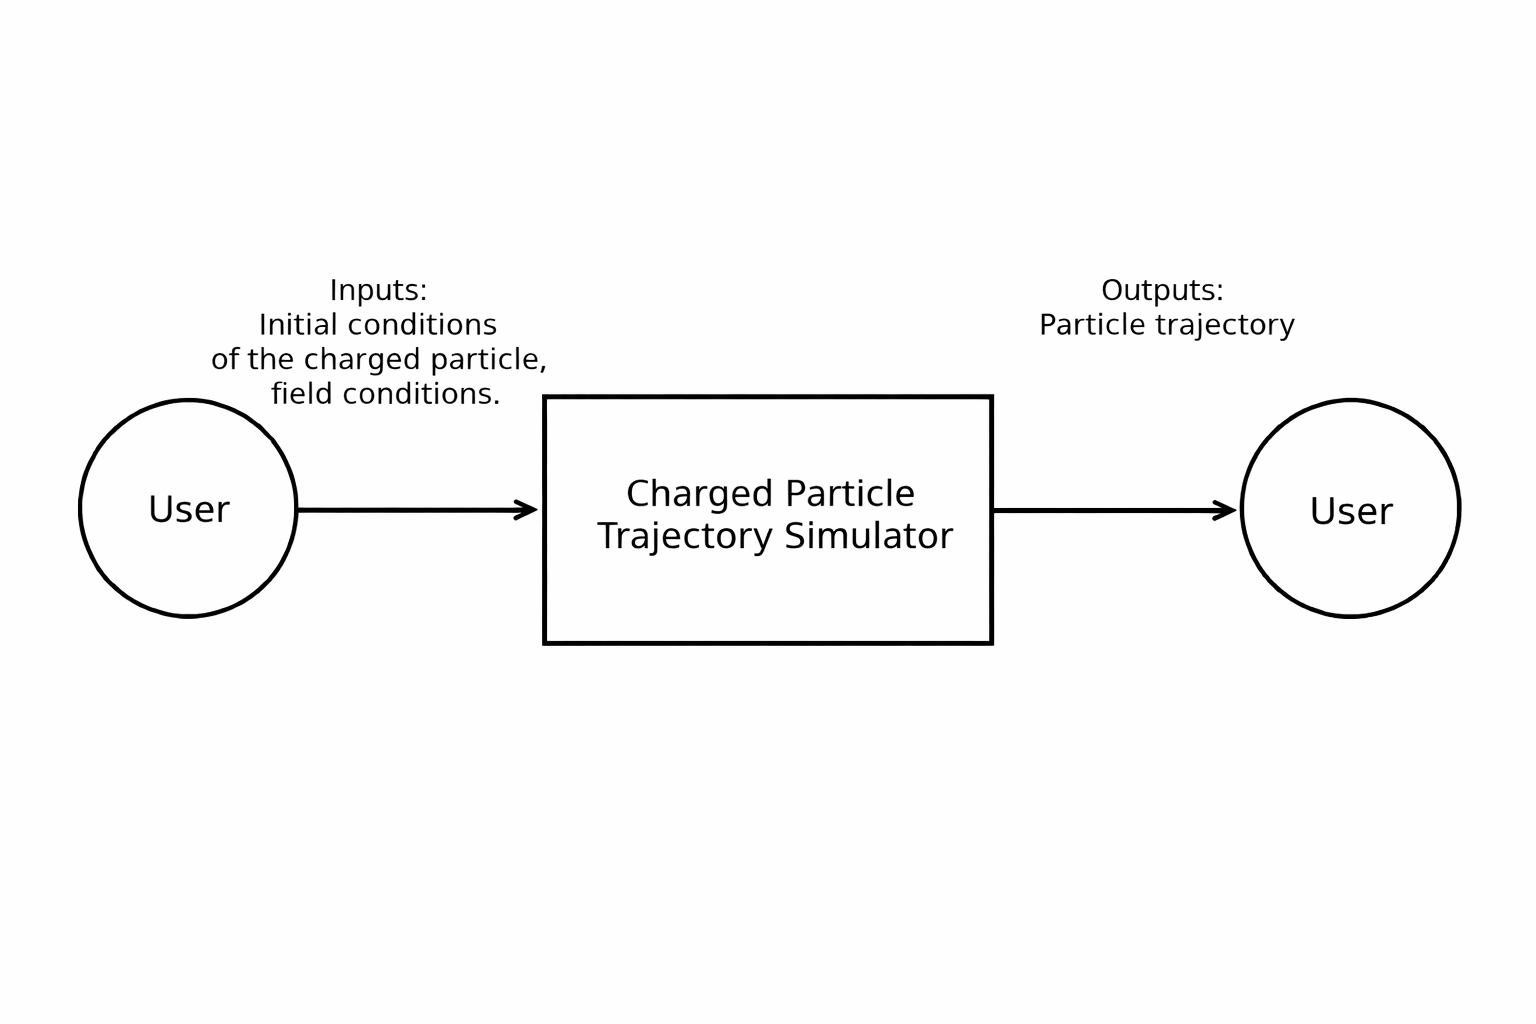
\includegraphics[width=0.9\textwidth]{diagram.jpg}%
}{%
  \fbox{Missing figure file diagram.jpg}%
}
\caption{System Context}
\label{Fig_SystemContext}
\end{center}
\end{figure}

The interaction between the product and the user is through a text-based
interface. The
responsibilities of the user and the system are as follows:

\begin{itemize}
\item User Responsibilities:
\begin{itemize}
\item Provide initial conditions of the physical state of the motion and the input data
  related to the projectile, ensuring no errors in the data entry.
\item Ensure that consistent units are used for input variables.
\item Ensure required software assumptions are appropriate for any particular problem input
  to the software.
\end{itemize}

\item \progname{} Responsibilities:
\begin{itemize}
\item Detect data type mismatch, such as a string of characters input instead of a
  floating point number.
\item Determine if the inputs satisfy the required physical and software constraints.
\item Calculate the required outputs.
\end{itemize}
\end{itemize}

\subsection{User Characteristics} \label{SecUserCharacteristics}

The end user of \progname{} should have an understanding of undergraduate-level physics
(including classical mechanics and introductory electromagnetism) and undergraduate-level
mathematics (including calculus and ordinary differential equations). Familiarity with
numerical methods or scientific computing is helpful but not required.

\subsection{System Constraints} \label{SecSysConstraints}

\progname{} requires Python~3.10 or later with NumPy, SciPy, and Matplotlib installed.


\section{Specific System Description}

This section first presents the problem description, which gives a high-level
view of the problem to be solved.  This is followed by the solution characteristics
specification, which presents the assumptions, theories, definitions and finally
the instance models.

\subsection{Problem Description} \label{Sec_pd}

\progname{} is intended to predict the projectile of charged particle in magnetic field.

\subsubsection{Terminology and  Definitions}

This subsection provides a list of terms that are used in the subsequent
sections and their meaning, with the purpose of reducing ambiguity and making it
easier to correctly understand the requirements:

\begin{itemize}

\item Charged particle: A particle that has a non-zero electric charge and can
interact with electric and magnetic fields.

\item Electric field: A physical field that exerts an electric force on charged
particles.

\item Magnetic field: A physical field that exerts a magnetic force on moving
charged particles.

\item Lorentz force: The force on a charged particle due to electric and
magnetic fields.

\item Trajectory: The path traced by a particle over time.

\item Field region: A spatial region in which the electric field and magnetic
field are specified (typically treated as uniform within the region).

\item Detector line: A line at a specified location where the particle impact
position is recorded.

\item Velocity selector: A configuration of crossed electric and magnetic fields
that allows only particles with a particular velocity to pass through without
deflection.

\item Projectile: The object to be launched at the target.

\item Cartesian coordinate system: A coordinate system that specifies each point uniquely in a plane by a set of numerical coordinates, which are the signed distances to the point from two fixed perpendicular oriented lines, measured in the same unit of length (from cartesianWiki).

\end{itemize}

\subsubsection{Physical System Description} \label{sec_phySystDescrip}

The physical system of \progname{}, as shown in
Figure~\ref{Fig_PhysicalSystem}, includes the following elements:

\begin{itemize}
\item[PS1:] The charged particle (with velocity $\mathbf{v}_0$, charge $q$ and mass $m$) at initial point $\mathbf{x}_0$.
\item[PS2:] The bounded region of uniform magnetic field $\mathbf{B}$ and electrc field $\mathbf{E}$.
\item[PS3:] The trajectory: the path traced by the charged particle as it travels through the field regions from $\mathbf{x}_0$ toward the detector plane.
\item[PS4:] The detector plane.
\item[PS5:] The impact point $x_{hit}$ on the detector plan.
\end{itemize}



\begin{figure}[h!]
\begin{center}
  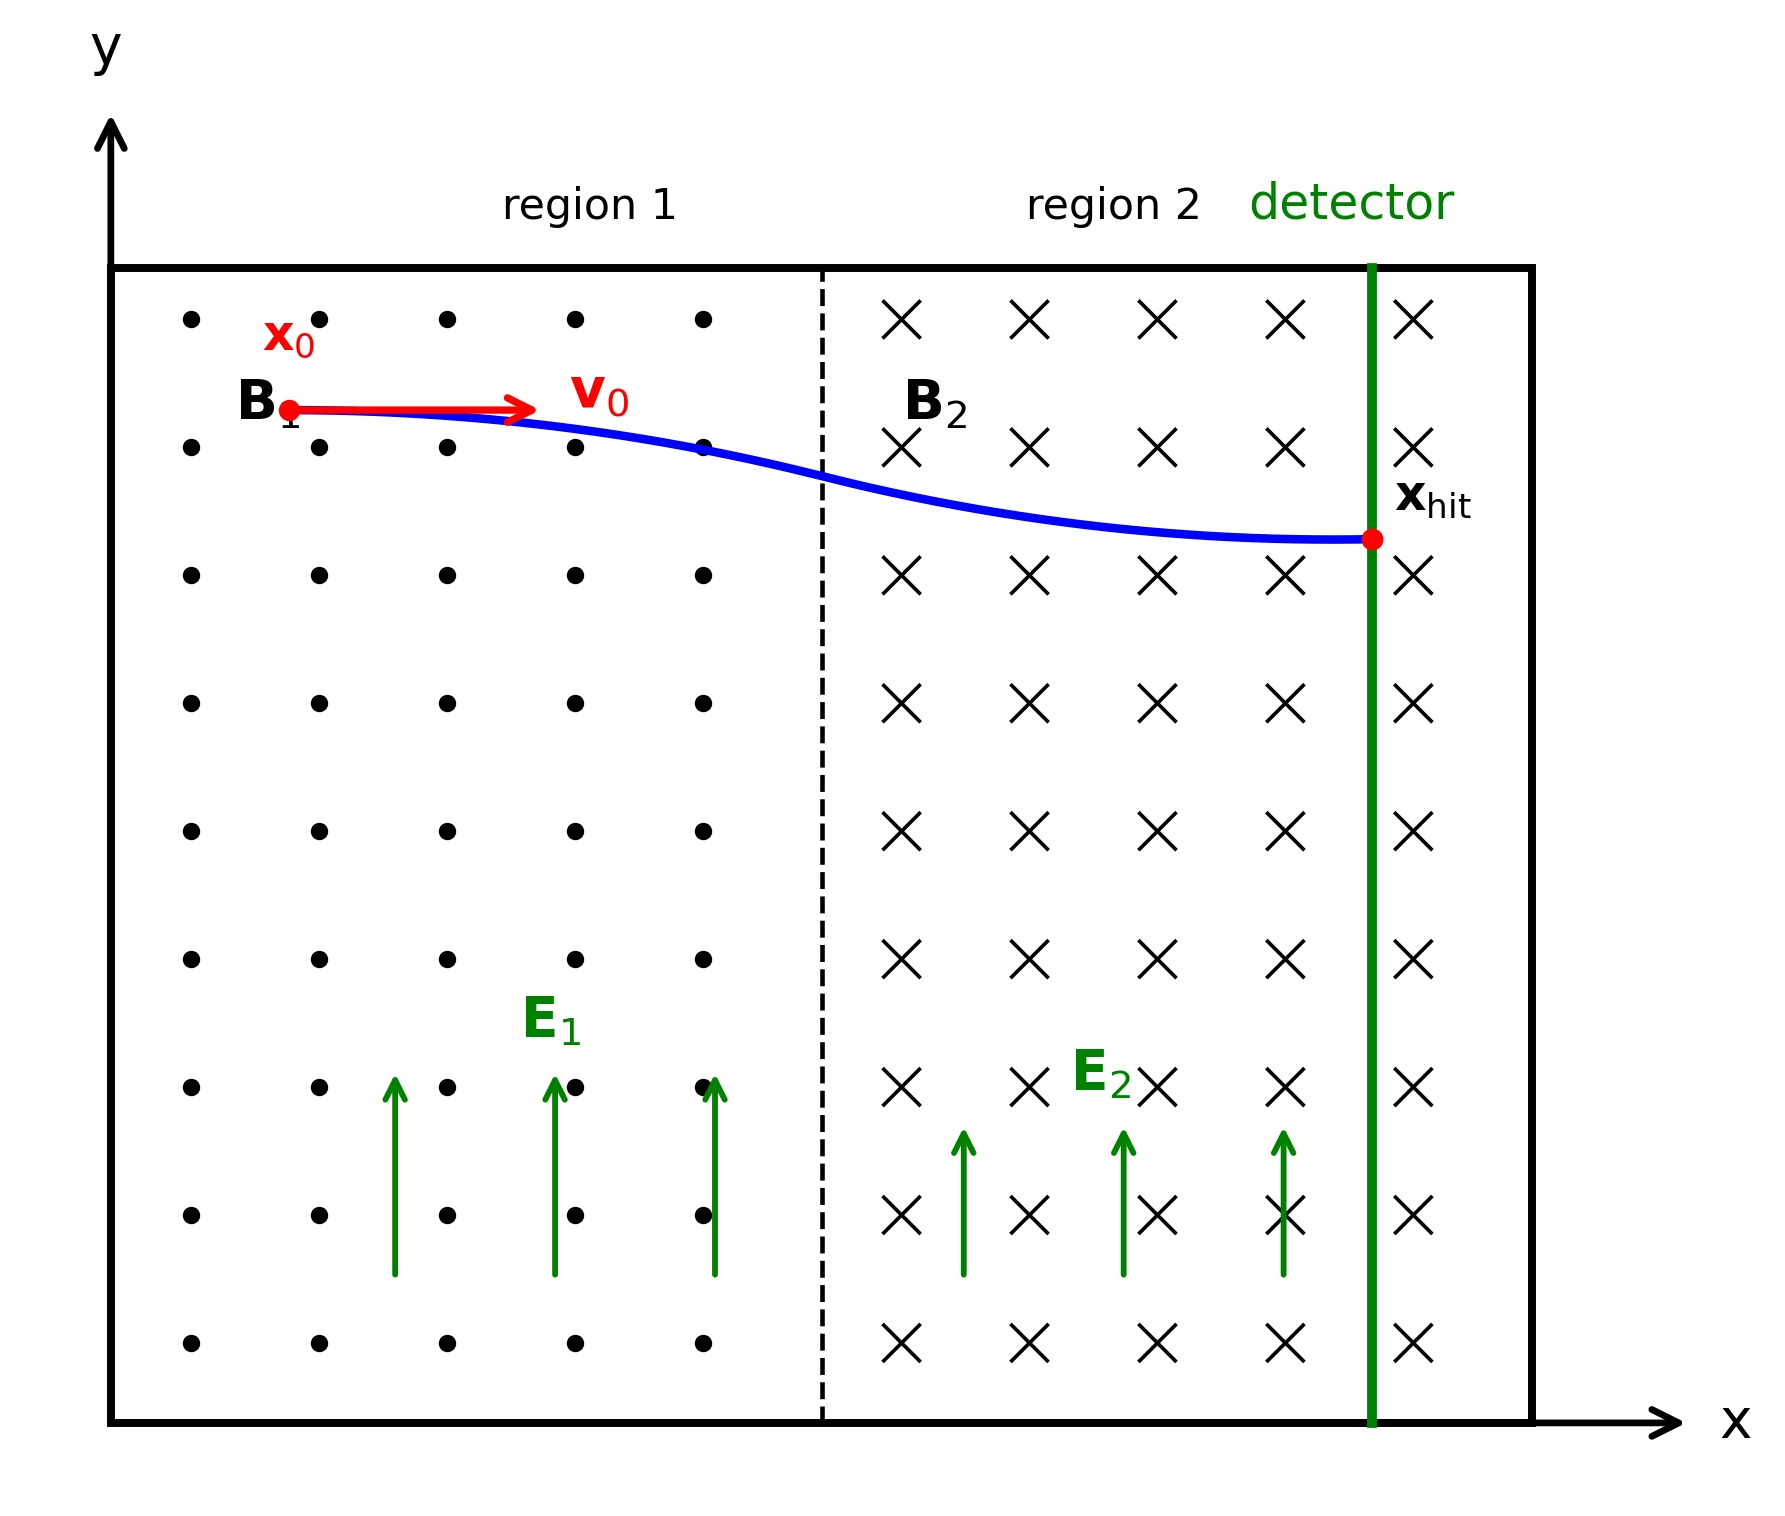
\includegraphics[width=0.85\textwidth]{figure2_multi_region_reversed_B.jpg}
\caption{The physical system.}
\label{Fig_PhysicalSystem}
\end{center}
\end{figure}


\subsubsection{Goal Statements}

\noindent Given the particle properties (charge and mass), initial conditions
(initial position and velocity), the specification of electric and magnetic
fields over one or more field regions, and the detector geometry, the goal
statements are:

\begin{itemize}

\item[GS\refstepcounter{goalnum}\thegoalnum \label{G_Trajectory}:]
Predict the trajectory of a charged particle under prescribed electric and magnetic fields.

\item[GS\refstepcounter{goalnum}\thegoalnum \label{G_DetectorOutcome}:]
Determine impact position and time-of-flight at a specified detector line.

\end{itemize}


\subsection{Solution Characteristics Specification}

This section first presents the problem description, which gives a high-level view of the problem to be solved. This is followed by the solution characteristics specification, which presents the assumptions, theories, and definitions that are used.

% \plt{This section specifies the information in the solution domain of the system
%   to be developed. This section is intended to express what is required in
%   such a way that analysts and stakeholders get a clear picture, and the
%   latter will accept it. The purpose of this section is to reduce the problem
%   into one expressed in mathematical terms. Mathematical expertise is used to
%   extract the essentials from the underlying physical description of the
%   problem, and to collect and substantiate all physical data pertinent to the
%   problem.}

% \plt{This section presents the solution characteristics by successively refining
%   models.  It starts with the abstract/general Theoretical Models (TMs) and
%   refines them to the concrete/specific Instance Models (IMs).  If necessary
%   there are intermediate refinements to General Definitions (GDs).  All of these
%   refinements can potentially use Assumptions (A) and Data Definitions (DD).
%   TMs are refined to create new models, that are called GMs or IMs. DDs are not
%   refined; they are just used. GDs and IMs are derived, or refined, from other
%   models. DDs are not derived; they are just given. TMs are also just given, but
%   they are refined, not used.  If a potential DD includes a derivation, then
%   that means it is refining other models, which would make it a GD or an IM.}

% \plt{The above makes a distinction between ``refined'' and ``used.'' A model is
%   refined to another model if it is changed by the refinement. When we change a
%   general 3D equation to a 2D equation, we are making a refinement, by applying
%   the assumption that the third dimension does not matter. If we use a
%   definition, like the definition of density, we aren't refining, or changing
%   that definition, we are just using it.}

% \plt{The same information can be a TM in one problem and a DD in another.  It is
%   about how the information is used.  In one problem the definition of
%   acceleration can be a TM, in another it would be a DD.}

% \plt{There is repetition between the information given in the different chunks
%   (TM, GDs etc) with other information in the document.  For instance, the
%   meaning of the symbols, the units etc are repeated.  This is so that the
%   chunks can stand on their own when being read by a reviewer/user.  It also
%   facilitates reuse of the models in a different context.}

% \noindent \plt{The relationships between the parts of the document are show in
%   the following figure.  In this diagram ``may ref'' has the same role as
%   ``uses'' above.  The figure adds ``Likely Changes,'' which are able to
%   reference (use) Assumptions.}

% \begin{figure}[H]
%   \IfFileExists{RelationsBetweenTM_GD_IM_DD_A.pdf}{%
%     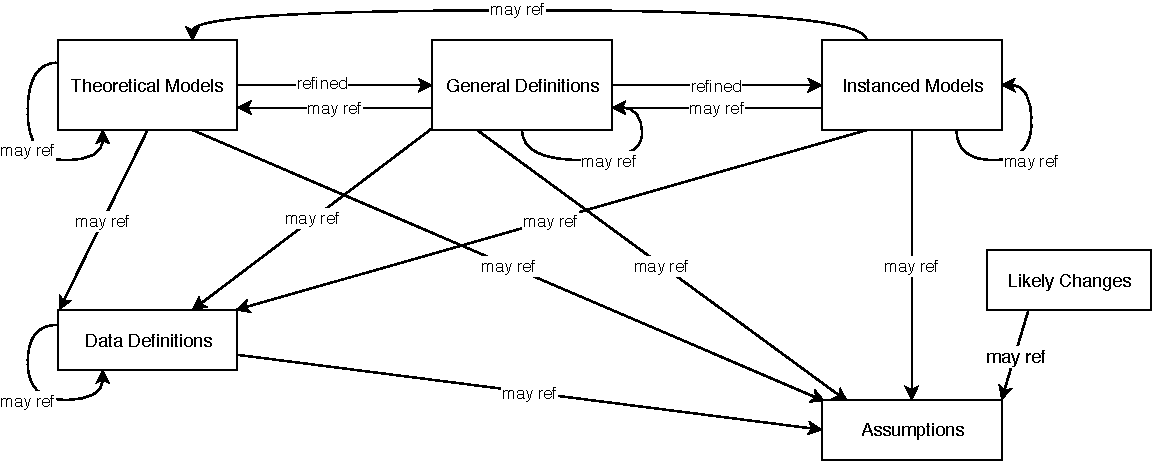
\includegraphics[scale=0.9]{RelationsBetweenTM_GD_IM_DD_A.pdf}%
%   }{%
%     \caption{(Placeholder) RelationsBetweenTM\_GD\_IM\_DD\_A.pdf not found.}%
%   }
% \end{figure}

The instance models that govern \progname{} are presented in
Subsection~\ref{sec_instance}.  The information to understand the meaning of the
instance models and their derivation is also presented, so that the instance
models can be verified.

\subsubsection{Types}

Not Applicable. Data type definitions are provided in Section~\ref{sec_datatypes}.

\subsubsection{Scope Decisions}

\begin{itemize}
\item \textbf{Two-dimensional motion:} The simulation is restricted to particle motion in the
  $x$--$y$ plane. Three-dimensional trajectories are outside the current scope and are listed
  as a likely change (\lcref{LC_3D}). This restriction matches common
  experimental configurations (e.g., cathode-ray tubes, mass spectrometers) and keeps the
  input specification and output interpretation straightforward.

\item \textbf{Single charged particle:} Only a single particle is simulated per run. Multi-particle
  beams and collective effects are out of scope.

\item \textbf{Classical (non-relativistic) dynamics:} Relativistic corrections are excluded.
  This is valid for particle speeds much less than the speed of light, which is the typical
  regime for the target educational and exploratory use cases.
\end{itemize}

\subsubsection{Modelling Decisions}

\begin{itemize}
\item \textbf{Cartesian coordinate system:} The particle position and velocity are represented in
  a Cartesian ($x$--$y$) coordinate system. This choice aligns naturally with rectangular
  field-region boundaries (\aref{A_rectRegions}), simplifies the component form of the equations
  of motion, and makes numerical implementation straightforward.

\item \textbf{Piecewise-uniform fields:} Electric and magnetic fields are modelled as spatially
  uniform within each rectangular region (\aref{A_piecewiseUniform}). This approximates real
  devices built from discrete uniform-field cells (e.g., parallel-plate capacitors, solenoid
  sections) and makes field specification explicit at region boundaries.

\item \textbf{Lorentz force only:} Particle dynamics are governed solely by the Lorentz force
  (\aref{A_lorentzOnly}). Gravity, radiation reaction, and other forces are negligible for the
  target use cases and are excluded to keep the model focused on electromagnetic physics.
\end{itemize}

\subsubsection{Physical Constants}

Not Applicable. No universal physical constants appear in the governing equations as fixed
parameters; all field values and particle properties are user-specified inputs.

\subsubsection{Assumptions} \label{sec_assumpt}

This section simplifies the original problem and helps in developing the
theoretical model by filling in the missing information for the physical system.
The numbers given in the square brackets refer to the theoretical model [TM],
general definition [GD], data definition [DD], instance model [IM], or likely
change [LC], in which the respective assumption is used.

\begin{itemize}

\item[A\refstepcounter{assumpnum}\theassumpnum \label{A_piecewiseUniform}:]
piecewiseUniform: The electric and magnetic fields are uniform within each field
region and may change only at region boundaries. [\ddref{DD_fieldsByRegion},
\iref{IM_stateEvol}, \rref{R_inputSpec}, \rref{R_computeTraj}, \lcref{LC_3D}]

\item[A\refstepcounter{assumpnum}\theassumpnum \label{A_singleParticle}:]
singleParticle: The particle is treated as a point mass and point charge.
[\tref{TM:newton2}, \tref{TM:lorentzForce}, \tref{TM:eqnMotion}, \iref{IM_stateEvol},
\rref{R_computeTraj}]

\item[A\refstepcounter{assumpnum}\theassumpnum \label{A_noInteractions}:]
noInteractions: Collisions and particle--particle interactions (including
space-charge effects) are neglected. [\iref{IM_stateEvol}, \rref{R_computeTraj}]

\item[A\refstepcounter{assumpnum}\theassumpnum \label{A_prescribedFields}:]
prescribedFields: The electric and magnetic fields are user-specified and remain
fixed during the simulation. [\tref{TM:lorentzForce}, \tref{TM:eqnMotion},
\dref{GD_dyn2D}, \ddref{DD_fieldsByRegion}, \iref{IM_stateEvol}, \rref{R_inputSpec},
\rref{R_computeTraj}]

\item[A\refstepcounter{assumpnum}\theassumpnum \label{A_twoDMotion}:]
twoDMotion: The particle motion is confined to the $x$--$y$ plane.
[\dref{GD_kin2D}, \dref{GD_vCrossB2D}, \dref{GD_dyn2D}, \iref{IM_stateEvol},
\rref{R_computeTraj}, \lcref{LC_3D}]

\item[A\refstepcounter{assumpnum}\theassumpnum \label{A_BperpPlane}:]
BperpPlane: The magnetic field is perpendicular to the $x$--$y$ plane.
[\dref{GD_vCrossB2D}, \dref{GD_dyn2D}, \ddref{DD_BField}, \iref{IM_stateEvol},
\rref{R_computeTraj}, \lcref{LC_3D}]

\item[A\refstepcounter{assumpnum}\theassumpnum \label{A_EaxisAligned}:]
EaxisAligned: The electric field lies in the $x$--$y$ plane and is aligned with a
coordinate axis. [\dref{GD_dyn2D}, \iref{IM_stateEvol}, \rref{R_computeTraj},
\lcref{LC_3D}]

\item[A\refstepcounter{assumpnum}\theassumpnum \label{A_rectRegions}:]
rectRegions: Field-region boundaries are rectangular and parallel to the $x$ and
$y$ axes. [\ddref{DD_regionRect}, \ddref{DD_fieldsByRegion}, \iref{IM_stateEvol},
\rref{R_inputSpec}, \rref{R_computeTraj}]

\item[A\refstepcounter{assumpnum}\theassumpnum \label{A_lineDetector}:]
lineDetector: The detector is modeled as a line located within the field region.
[\ddref{DD_detectorLine}, \iref{IM_detHit}, \rref{R_inputSpec}, \rref{R_detectHit}]

\item[A\refstepcounter{assumpnum}\theassumpnum \label{A_fullDetection}:]
fullDetection: The detector line is sufficiently long to record the impact point
for any trajectory within the scope of the simulation.
[\ddref{DD_detectorLine}, \iref{IM_detHit}, \rref{R_inputSpec}, \rref{R_detectHit}]

\item[A\refstepcounter{assumpnum}\theassumpnum \label{A_lorentzOnly}:]
lorentzOnly: The particle dynamics are governed only by the Lorentz force; all
other forces are neglected. [\tref{TM:eqnMotion}, \iref{IM_stateEvol},
\rref{R_computeTraj}]

\end{itemize}



\subsubsection{Theoretical Models}\label{sec_theoretical}

This section focuses on the general equations and laws that \progname{} is based
on.

\noindent
\deftheory
{TM:velVec}
{Velocity (vector definition)}
{
  $\mathbf{v}(t) = \dfrac{d\mathbf{r}(t)}{dt}$
}
{
  $\mathbf{v}(t)$ is the particle velocity (\si{\metre\per\second}),
  $\mathbf{r}(t)$ is the particle position (\si{\metre}), and
  $t$ is time (\si{\second}).
}
{None.}
{\cite{WikiVelocity}}
{\dref{GD_kin2D}}
{None.}
{}


\noindent
\deftheory
{TM:accVec}
{Acceleration (vector definition)}
{
  $\mathbf{a}(t) = \dfrac{d\mathbf{v}(t)}{dt}$
}
{
  $\mathbf{a}(t)$ is the particle acceleration (\si{\metre\per\second\squared}),
  $\mathbf{v}(t)$ is the particle velocity (\si{\metre\per\second}), and
  $t$ is time (\si{\second}).
}
{None.}
{\cite{WikiAcceleration}}
{\tref{TM:newton2}, \tref{TM:eqnMotion}}
{None.}
{}


\noindent
\deftheory
{TM:newton2}
{Newton's second law of motion}
{
  $\mathbf{F}(t) = m\,\mathbf{a}(t)$
}
{
  $\mathbf{F}(t)$ is the net force on the particle (\si{\newton}),
  $m$ is the particle mass (\si{\kilogram}), and
  $\mathbf{a}(t)$ is the particle acceleration (\si{\metre\per\second\squared}).
}
{
  The net force on a body is proportional to its acceleration, where $m$ is the
  constant of proportionality.
}
{\cite{WikiAcceleration}}
{\tref{TM:eqnMotion}}
{\aref{A_singleParticle}}
{}


\noindent
\deftheory
{TM:lorentzForce}
{Lorentz force law}
{
  $\mathbf{F}(t) = q\left(\mathbf{E} + \mathbf{v}(t)\times\mathbf{B}\right)$
}
{
  $\mathbf{F}(t)$ is the electromagnetic force on the particle (\si{\newton}),
  $q$ is the particle charge (\si{\coulomb}),
  $\mathbf{E}$ is the electric field (\si{\newton\per\coulomb}),
  $\mathbf{B}$ is the magnetic flux density (\si{\tesla}), and
  $\mathbf{v}(t)$ is the particle velocity (\si{\metre\per\second}).
}
{None.}
{\cite{WikiElectromagnetism}}
{\tref{TM:eqnMotion}, \dref{GD_dyn2D}}
{\aref{A_singleParticle}, \aref{A_prescribedFields}}
{}


\noindent
\deftheory
{TM:eqnMotion}
{Equation of motion under electromagnetic fields}
{
  $m\,\dfrac{d\mathbf{v}(t)}{dt} = q\left(\mathbf{E} + \mathbf{v}(t)\times\mathbf{B}\right)$
}
{
  This equation combines \tref{TM:newton2} (Newton's second law) with
  \tref{TM:lorentzForce} (Lorentz force law), using the definition of acceleration
  \tref{TM:accVec}, to yield the governing ordinary differential equation (ODE) for
  the particle velocity $\mathbf{v}(t)$ under the specified electric and magnetic fields.
}
{None.}
{\cite{WikiElectromagnetism}}
{\dref{GD_dyn2D}, \iref{IM_stateEvol}}
{\aref{A_singleParticle}, \aref{A_prescribedFields}, \aref{A_lorentzOnly}}
{}

~\newline


\subsubsection{General Definitions}\label{sec_gendef}

This section collects the laws and equations that will be used in building the
instance models.

~\newline

\noindent
\begin{minipage}{\textwidth}
\renewcommand*{\arraystretch}{1.5}
\begin{tabular}{| p{\colAwidth} | p{\colBwidth}|}
\hline
\rowcolor[gray]{0.9}
Number& GD\refstepcounter{defnum}\thedefnum \label{GD_kin2D}\\
\hline
Label &\bf Two-dimensional kinematics in Cartesian coordinates \\
\hline
Units& \si{\metre\per\second}\\
\hline
Equation&
$\dfrac{dx(t)}{dt} = v_x(t), \quad \dfrac{dy(t)}{dt} = v_y(t)$ \\
\hline
Description &
The planar motion assumption (\aref{A_twoDMotion}) allows the particle position
to be represented by $(x(t),y(t))$ and the velocity by $(v_x(t),v_y(t))$ in a
Cartesian coordinate system. The equations define the velocity components as the
time-derivatives of the corresponding position components.\\
\hline
Source & None\\
\hline
Ref.\ By & \iref{IM_stateEvol}\\
\hline
\end{tabular}
\end{minipage}\\

\subsubsection*{Detailed derivation of two-dimensional kinematics}
Let $\mathbf{r}(t) = \langle x(t), y(t), 0\rangle$ and $\mathbf{v}(t) =
\dfrac{d\mathbf{r}(t)}{dt}$ (from \tref{TM:velVec}). Taking components yields
$\dfrac{dx(t)}{dt} = v_x(t)$ and $\dfrac{dy(t)}{dt} = v_y(t)$.

~\newline


\noindent
\begin{minipage}{\textwidth}
\renewcommand*{\arraystretch}{1.5}
\begin{tabular}{| p{\colAwidth} | p{\colBwidth}|}
\hline
\rowcolor[gray]{0.9}
Number& GD\refstepcounter{defnum}\thedefnum \label{GD_vCrossB2D}\\
\hline
Label &\bf Cross product $\mathbf{v}\times\mathbf{B}$ for out-of-plane magnetic field \\
\hline
Units& \si{\metre\per\second}\,\si{\tesla}\\
\hline
Equation&
$\mathbf{v}(t)\times\mathbf{B} = \langle v_y(t)B,\; -v_x(t)B,\; 0\rangle$ \\
\hline
Description &
Under planar motion (\aref{A_twoDMotion}) and an out-of-plane magnetic field
(\aref{A_BperpPlane}), the velocity has the form
$\mathbf{v}(t)=\langle v_x(t),v_y(t),0\rangle$ and the magnetic field has the
form $\mathbf{B}=\langle 0,0,B\rangle$. The cross product then reduces to the
stated component form.\\
\hline
Source & None\\
\hline
Ref.\ By & \dref{GD_dyn2D}\\
\hline
\end{tabular}
\end{minipage}\\

\subsubsection*{Detailed derivation of $\mathbf{v}\times\mathbf{B}$ in 2D}
With $\mathbf{v}(t)=\langle v_x(t),v_y(t),0\rangle$ and
$\mathbf{B}=\langle 0,0,B\rangle$,
\[
\mathbf{v}(t)\times\mathbf{B} =
\begin{vmatrix}
\mathbf{i} & \mathbf{j} & \mathbf{k}\\
v_x(t) & v_y(t) & 0\\
0 & 0 & B
\end{vmatrix}
= \langle v_y(t)B,\; -v_x(t)B,\; 0\rangle .
\]

~\newline

\noindent
\begin{minipage}{\textwidth}
\renewcommand*{\arraystretch}{1.5}
\begin{tabular}{| p{\colAwidth} | p{\colBwidth}|}
\hline
\rowcolor[gray]{0.9}
Number& GD\refstepcounter{defnum}\thedefnum \label{GD_dyn2D}\\
\hline
Label &\bf Two-dimensional equations of motion under $\mathbf{E}$ and $\mathbf{B}$ \\
\hline
Units& \si{\metre\per\second\squared}\\
\hline
Equation&
$\dfrac{dv_x(t)}{dt} = \dfrac{q}{m}\big(E_x + v_y(t)B\big), \quad
 \dfrac{dv_y(t)}{dt} = \dfrac{q}{m}\big(E_y - v_x(t)B\big)$ \\
\hline
Description &
Assuming planar motion (\aref{A_twoDMotion}), prescribed fields (\aref{A_prescribedFields}),
and an out-of-plane magnetic field (\aref{A_BperpPlane}), the Lorentz-force
equation of motion (\tref{TM:eqnMotion}) can be written component-wise in the
$x$--$y$ plane. Here $\mathbf{E}=\langle E_x,E_y,0\rangle$ and
$\mathbf{B}=\langle 0,0,B\rangle$, yielding the stated ODEs for $v_x(t)$ and
$v_y(t)$.\\
\hline
Source & None\\
\hline
Ref.\ By & \iref{IM_stateEvol}\\
\hline
\end{tabular}
\end{minipage}\\

\subsubsection*{Detailed derivation of the 2D equations of motion}
From Newton's second law (\tref{TM:newton2}) and the Lorentz force law
(\tref{TM:lorentzForce}),
\[
m\,\dfrac{d\mathbf{v}(t)}{dt} = q\left(\mathbf{E} + \mathbf{v}(t)\times\mathbf{B}\right).
\]
Using $\mathbf{E}=\langle E_x,E_y,0\rangle$ and the 2D cross product reduction
(\dref{GD_vCrossB2D}),
\[
\mathbf{E} + \mathbf{v}(t)\times\mathbf{B}
= \langle E_x + v_y(t)B,\; E_y - v_x(t)B,\; 0\rangle .
\]
Equating components gives
\[
m\,\dfrac{dv_x(t)}{dt} = q\big(E_x + v_y(t)B\big), \quad
m\,\dfrac{dv_y(t)}{dt} = q\big(E_y - v_x(t)B\big),
\]
and dividing by $m$ yields the stated ODEs.


\subsubsection{Data Definitions}\label{sec_datadef}

This section collects and defines all the data needed to build the instance
models.

~\newline


\noindent
\begin{minipage}{\textwidth}
\renewcommand*{\arraystretch}{1.5}
\begin{tabular}{| p{\colAwidth} | p{\colBwidth}|}
\hline
\rowcolor[gray]{0.9}
Number& DD\refstepcounter{datadefnum}\thedatadefnum \label{DD_qOverm}\\
\hline
Label& \bf Charge-to-mass ratio\\
\hline
Symbol &$\kappa$\\
\hline
Units & \si{\coulomb\per\kilogram}\\
\hline
Equation& $\kappa = \dfrac{q}{m}$\\
\hline
Description &
$q$ is the particle charge (\si{\coulomb}) and $m$ is the particle mass
(\si{\kilogram}). The ratio $\kappa$ is used to simplify the equations of motion.
\\
\hline
Sources& None\\ \hline
Ref.\ By & \iref{IM_stateEvol}\\ \hline
\end{tabular}
\end{minipage}\\

~\newline


\noindent
\begin{minipage}{\textwidth}
\renewcommand*{\arraystretch}{1.5}
\begin{tabular}{| p{\colAwidth} | p{\colBwidth}|}
\hline
\rowcolor[gray]{0.9}
Number& DD\refstepcounter{datadefnum}\thedatadefnum \label{DD_initState}\\
\hline
Label& \bf Initial state in the $x$--$y$ plane\\
\hline
Symbol &$\mathbf{s}_0$\\
\hline
Units & \si{\metre}, \si{\metre\per\second}\\
\hline
Equation& $\mathbf{s}_0 = \langle x_0,\; y_0,\; v_{0x},\; v_{0y}\rangle$\\
\hline
Description &
$x_0,y_0$ are the initial position components (\si{\metre}) and
$v_{0x},v_{0y}$ are the initial velocity components (\si{\metre\per\second}).
\\
\hline
Sources& None\\ \hline
Ref.\ By & \iref{IM_stateEvol}\\ \hline
\end{tabular}
\end{minipage}\\

~\newline


\noindent
\begin{minipage}{\textwidth}
\renewcommand*{\arraystretch}{1.5}
\begin{tabular}{| p{\colAwidth} | p{\colBwidth}|}
\hline
\rowcolor[gray]{0.9}
Number& DD\refstepcounter{datadefnum}\thedatadefnum \label{DD_EField}\\
\hline
Label& \bf Electric field vector\\
\hline
Symbol &$\mathbf{E}$\\
\hline
Units & \si{\newton\per\coulomb}\\
\hline
Equation& $\mathbf{E}=\langle E_x,\; E_y,\; 0\rangle$\\
\hline
Description &
$\mathbf{E}$ is the electric field. $E_x$ and $E_y$ are the in-plane components
(\si{\newton\per\coulomb}).
\\
\hline
Sources& None\\ \hline
Ref.\ By & \ddref{DD_fieldsByRegion}, \dref{GD_dyn2D}\\ \hline
\end{tabular}
\end{minipage}\\

~\newline


\noindent
\begin{minipage}{\textwidth}
\renewcommand*{\arraystretch}{1.5}
\begin{tabular}{| p{\colAwidth} | p{\colBwidth}|}
\hline
\rowcolor[gray]{0.9}
Number& DD\refstepcounter{datadefnum}\thedatadefnum \label{DD_BField}\\
\hline
Label& \bf Magnetic flux density vector\\
\hline
Symbol &$\mathbf{B}$\\
\hline
Units & \si{\tesla}\\
\hline
Equation& $\mathbf{B}=\langle 0,\;0,\;B\rangle$\\
\hline
Description &
$\mathbf{B}$ is the magnetic flux density. $B$ is the out-of-plane component
(\si{\tesla}).
\\
\hline
Sources& None\\ \hline
Ref.\ By & \ddref{DD_fieldsByRegion}, \dref{GD_vCrossB2D}, \dref{GD_dyn2D}\\ \hline
\end{tabular}
\end{minipage}\\

~\newline


\noindent
\begin{minipage}{\textwidth}
\renewcommand*{\arraystretch}{1.5}
\begin{tabular}{| p{\colAwidth} | p{\colBwidth}|}
\hline
\rowcolor[gray]{0.9}
Number& DD\refstepcounter{datadefnum}\thedatadefnum \label{DD_regionRect}\\
\hline
Label& \bf Rectangular field region\\
\hline
Symbol &$R_i$\\
\hline
Units & \si{\metre}\\
\hline
Equation&
$R_i = [x^{(i)}_{\min},x^{(i)}_{\max}]\times[y^{(i)}_{\min},y^{(i)}_{\max}]$\\
\hline
Description &
$R_i$ is the $i$th field region. The parameters
$x^{(i)}_{\min},x^{(i)}_{\max},y^{(i)}_{\min},y^{(i)}_{\max}$ define the region
boundaries in the $x$--$y$ plane (all in \si{\metre}).
\\
\hline
Sources& None\\ \hline
Ref.\ By & \ddref{DD_fieldsByRegion}\\ \hline
\end{tabular}
\end{minipage}\\

~\newline

%--------------------------------------------------------------------
% DD 6: piecewise-constant fields by region
%--------------------------------------------------------------------
\noindent
\begin{minipage}{\textwidth}
\renewcommand*{\arraystretch}{1.5}
\begin{tabular}{| p{\colAwidth} | p{\colBwidth}|}
\hline
\rowcolor[gray]{0.9}
Number& DD\refstepcounter{datadefnum}\thedatadefnum \label{DD_fieldsByRegion}\\
\hline
Label& \bf Piecewise-constant fields\\
\hline
Symbol & $\mathbf{E}_i,\mathbf{B}_i$\\
\hline
Units & \si{\newton\per\coulomb}, \si{\tesla}\\
\hline
Equation&
$\mathbf{E}(\mathbf{r})=\mathbf{E}_i,\ \mathbf{B}(\mathbf{r})=\mathbf{B}_i,\ \forall \mathbf{r}\in R_i$\\
\hline
Description &
$\mathbf{E}_i$ and $\mathbf{B}_i$ are the constant electric and magnetic field
values assigned to region $R_i$. The fields may differ between regions.
\\
\hline
Sources& None\\ \hline
Ref.\ By & \iref{IM_stateEvol}\\ \hline
\end{tabular}
\end{minipage}\\

~\newline

%--------------------------------------------------------------------
% DD 7: detector line
%--------------------------------------------------------------------
\noindent
\begin{minipage}{\textwidth}
\renewcommand*{\arraystretch}{1.5}
\begin{tabular}{| p{\colAwidth} | p{\colBwidth}|}
\hline
\rowcolor[gray]{0.9}
Number& DD\refstepcounter{datadefnum}\thedatadefnum \label{DD_detectorLine}\\
\hline
Label& \bf Detector line\\
\hline
Symbol &$L_{\mathrm{det}}$\\
\hline
Units & $(\si{\metre},\si{\metre})$\\
\hline
Equation&
$L_{\mathrm{det}}=\{(x,y)\ |\ x=x_{\mathrm{det}},\ y\in[y_{\min}^{\mathrm{det}},y_{\max}^{\mathrm{det}}]\}$\\
\hline
Description &
$L_{\mathrm{det}}$ is the detector line segment located at $x=x_{\mathrm{det}}$.
The endpoints are defined by $y_{\min}^{\mathrm{det}}$ and $y_{\max}^{\mathrm{det}}$
(all in \si{\metre}).
\\
\hline
Sources& None\\ \hline
Ref.\ By & \iref{IM_detHit}\\ \hline
\end{tabular}
\end{minipage}\\


\subsubsection{Data Types}\label{sec_datatypes}

The standard real-number and vector types used in undergraduate physics and calculus are sufficient; no additional data types need to be defined for this problem.


\subsubsection{Instance Models} \label{sec_instance}

This section transforms the problem defined in Section~\ref{Sec_pd} into
one which is expressed in mathematical terms. It uses concrete symbols defined
in Section~\ref{sec_datadef} to replace the abstract symbols in the models
identified in Sections~\ref{sec_theoretical} and~\ref{sec_gendef}.

The goals \gsref{G_Trajectory} and \gsref{G_DetectorOutcome}
are solved by \iref{IM_stateEvol} and \iref{IM_detHit},
respectively. The instance models are derived from the equation of motion
(\tref{TM:eqnMotion}) and the general definitions (\dref{GD_kin2D}, \dref{GD_dyn2D})
under the assumptions in Section~\ref{sec_assumpt}.

~\newline

%--------------------------------------------------------------------
% Instance Model 1: state evolution under piecewise-uniform fields
%--------------------------------------------------------------------
\noindent
\begin{minipage}{\textwidth}
\renewcommand*{\arraystretch}{1.5}
\begin{tabular}{| p{\colAwidth} | p{\colBwidth}|}
  \hline
  \rowcolor[gray]{0.9}
  Number& IM\refstepcounter{instnum}\theinstnum \label{IM_stateEvol}\\
  \hline
  Label& \bf Particle state evolution in the $x$--$y$ plane\\
  \hline
  Input&
  $m, q, x_0, y_0, v_{0x}, v_{0y}, \{R_i\}_{i=1..N}, \{\mathbf{E}_i\}_{i=1..N}, \{\mathbf{B}_i\}_{i=1..N}, t_{\text{final}}$\\
  & Constraints: $m>0$, $q\neq 0$, $t_{\text{final}}>0$, and each $R_i$ is a non-degenerate axis-aligned rectangle.\\
  \hline
  Output&
  $\mathbf{s}(t)=\langle x(t),y(t),v_x(t),v_y(t)\rangle$ for $0\le t\le t_{\text{final}}$,
  such that\\
  & $\dfrac{dx}{dt} = v_x(t)$, \quad $\dfrac{dy}{dt} = v_y(t)$,\\
  & $\dfrac{dv_x}{dt} = \kappa\left(E_x(t) + v_y(t)\,B(t)\right)$,\\
  & $\dfrac{dv_y}{dt} = \kappa\left(E_y(t) - v_x(t)\,B(t)\right)$,\\
  & with initial condition $\mathbf{s}(0)=\langle x_0,y_0,v_{0x},v_{0y}\rangle$.\\
  \hline
  Description&
  Bold symbols (e.g., $\mathbf{s}$, $\mathbf{E}$, $\mathbf{B}$) denote vectors; the
  bold state vector $\mathbf{s}(t)=\langle x(t),y(t),v_x(t),v_y(t)\rangle$ collects
  position and velocity components.\\
  & $\kappa = q/m$ is the charge-to-mass ratio.\\
  & $(E_x(t),E_y(t))$ and $B(t)$ are determined by which region $R_i$ contains $(x(t),y(t))$:\\
  & if $(x(t),y(t))\in R_i$, then $\mathbf{E}(t)=\mathbf{E}_i=\langle E_x,E_y,0\rangle$
    and $\mathbf{B}(t)=\mathbf{B}_i=\langle 0,0,B\rangle$.\\
  & If $(x(t),y(t))$ lies outside all defined regions, the fields default to zero
  ($\mathbf{E}=\mathbf{0}$, $\mathbf{B}=\mathbf{0}$) and the particle undergoes free
  (force-free) motion in that area.\\
  & The model supports $E$-only, $B$-only, and crossed-field configurations by allowing
  $\mathbf{E}_i=\mathbf{0}$ and/or $\mathbf{B}_i=\mathbf{0}$ in any region.\\
  \hline
  Sources& None\\
  \hline
  Ref.\ By & None\\
  \hline
\end{tabular}
\end{minipage}\\

\subsubsection*{Derivation of \iref{IM_stateEvol}}
The governing ODE for the velocity is given by the equation of motion under electromagnetic
fields (\tref{TM:eqnMotion}). Under planar motion and the specified field orientations
(\aref{A_twoDMotion}, \aref{A_BperpPlane}, \aref{A_EaxisAligned}), the component form of
the dynamics is captured by \dref{GD_dyn2D}. The kinematic relations between position and
velocity components are given by \dref{GD_kin2D}. Combining \dref{GD_dyn2D} with
\dref{GD_kin2D}, and using $\kappa=q/m$ (\ddref{DD_qOverm}), yields the coupled first-order
ODE system in \iref{IM_stateEvol}. Piecewise-uniform regions and fixed user-specified fields
(\aref{A_piecewiseUniform}, \aref{A_prescribedFields}, \aref{A_rectRegions}) determine how
$\mathbf{E}(t)$ and $\mathbf{B}(t)$ are selected during the evolution.

~\newline

%--------------------------------------------------------------------
% Instance Model 2: first detector hit
%--------------------------------------------------------------------
\noindent
\begin{minipage}{\textwidth}
\renewcommand*{\arraystretch}{1.5}
\begin{tabular}{| p{\colAwidth} | p{\colBwidth}|}
  \hline
  \rowcolor[gray]{0.9}
  Number& IM\refstepcounter{instnum}\theinstnum \label{IM_detHit}\\
  \hline
  Label& \bf First detector intersection (hit time and hit location)\\
  \hline
  Input&
  $x_{\mathrm{det}}, y_{\min}^{\mathrm{det}}, y_{\max}^{\mathrm{det}}, x(t), y(t), t_{\text{final}}$\\
  & Constraints: $y_{\min}^{\mathrm{det}}<y_{\max}^{\mathrm{det}}$ and $0\le t\le t_{\text{final}}$.\\
  \hline
  Output&
  $t_{\mathrm{hit}}$ and $(x_{\mathrm{hit}},y_{\mathrm{hit}})$ such that\\
  & $t_{\mathrm{hit}} = \min\{t\in[0,t_{\text{final}}]\;|\;x(t)=x_{\mathrm{det}}
  \ \land\ y(t)\in[y_{\min}^{\mathrm{det}},y_{\max}^{\mathrm{det}}]\}$,\\
  & $x_{\mathrm{hit}} = x_{\mathrm{det}}$, \quad $y_{\mathrm{hit}} = y(t_{\mathrm{hit}})$.\\
  \hline
  Description&
  The detector is modeled as a vertical line segment at $x=x_{\mathrm{det}}$ with endpoints
  $y_{\min}^{\mathrm{det}}$ and $y_{\max}^{\mathrm{det}}$.\\
  & If the set defining $t_{\mathrm{hit}}$ is empty, then no detector hit occurs within
  $[0,t_{\text{final}}]$.\\
  \hline
  Sources& None\\
  \hline
  Ref.\ By & None\\
  \hline
\end{tabular}
\end{minipage}\\

\subsubsection*{Derivation of \iref{IM_detHit}}
The detector geometry is defined as a line segment (\ddref{DD_detectorLine}). The computed
trajectory $(x(t),y(t))$ is provided by \iref{IM_stateEvol}. The detector hit is the earliest
time at which the trajectory satisfies the detector-line condition and lies within the detector
segment bounds. This event definition yields the expression for $t_{\mathrm{hit}}$ and the
corresponding hit point $(x_{\mathrm{hit}},y_{\mathrm{hit}})$.

~\newline





\subsubsection{Data Constraints} \label{sec_DataConstraints}

The Input Data Constraints Table shows the data constraints on the input
variables. The column for physical constraints gives the physical limitations on
the range of values that can be taken by the variable. The uncertainty column
provides an estimate of the confidence with which the physical quantities can be
measured. This information would be part of the input if one were performing an
uncertainty quantification exercise. The constraints are conservative to give
the user of the model the flexibility to experiment with unusual situations. The
column of typical values is intended to provide a feel for a common scenario.

\begin{table}[!h]
\caption{Input Data Constraints} \label{TblInputVar}
\renewcommand{\arraystretch}{1.2}
\noindent \begin{longtable*}{l l l l l}
  \toprule
  \textbf{Var} & \textbf{Physical Constraints} & \textbf{Software Constraints} & \textbf{Typical Value} & \textbf{Uncert.} \\
  \midrule
  $m$ &
  $m > 0$ &
  $m_{\min} \le m \le m_{\max}$ &
  $9.11\times 10^{-31}\ \si{\kilogram}$ &
  $10\%$
  \\
  $q$ &
  $q \neq 0$ &
  $|q| \le q_{\max}$ &
  $-1.60\times 10^{-19}\ \si{\coulomb}$ &
  $10\%$
  \\
  $(x_0,y_0)$ &
  $(x_0,y_0)\in R_1$ &
  Within simulation domain &
  $(0,0)\ \si{\metre}$ &
  $0\%$
  \\
  $v_0$ &
  $v_0 > 0$ &
  $v_0 \le v_{\max}$ &
  $1.0\times 10^{6}\ \si{\metre\per\second}$ &
  $10\%$
  \\
  $R_i$ &
  $x^{(i)}_{\min} < x^{(i)}_{\max}$,\ $y^{(i)}_{\min} < y^{(i)}_{\max}$ &
  Non-degenerate rectangle &
  $0.10\times 0.10\ \si{\metre^2}$ &
  $0\%$
  \\
  $\mathbf{E}_i$ &
  Finite real-valued field &
  $|\mathbf{E}_i| \le E_{\max}$ &
  $1.0\times 10^{3}\ \si{\newton\per\coulomb}$ &
  $10\%$
  \\
  $\mathbf{B}_i$ &
  Finite real-valued field &
  $|B_i| \le B_{\max}$ &
  $1.0\times 10^{-2}\ \si{\tesla}$ &
  $10\%$
  \\
  $L_{\mathrm{det}}$ &
  $y^{\mathrm{det}}_{\min} < y^{\mathrm{det}}_{\max}$ &
  $x_{\mathrm{det}}$ within domain &
  $x_{\mathrm{det}} = 0.08\ \si{\metre}$ &
  $0\%$
  \\
  $t_{\text{final}}$ &
  $t_{\text{final}} > 0$ &
  $t_{\text{final}} \le t_{\max}$ &
  $1.0\times 10^{-6}\ \si{\second}$ &
  $10\%$
  \\
  \bottomrule
\end{longtable*}
\end{table}

\subsubsection{Properties of a Correct Solution} \label{sec_CorrectSolution}

\noindent
A correct solution must exhibit physically meaningful output values and known
constraints implied by the model structure (for instance, event definitions and
invariants in special cases). These properties are in addition to the stated
requirements.

\begin{table}[!h]
\caption{Output Data Constraints} \label{TblOutputVar}
\renewcommand{\arraystretch}{1.2}
\noindent \begin{longtable*}{l l}
  \toprule
  \textbf{Var} & \textbf{Physical Constraints} \\
  \midrule
  $t_{\mathrm{hit}}$ &
  $0 \le t_{\mathrm{hit}} \le t_{\text{final}}$ (if a hit occurs)
  \\
  $(x_{\mathrm{hit}},y_{\mathrm{hit}})$ &
  $x_{\mathrm{hit}} = x_{\mathrm{det}}$ and
  $y^{\mathrm{det}}_{\min} \le y_{\mathrm{hit}} \le y^{\mathrm{det}}_{\max}$ (if a hit occurs)
  \\
  $\Delta y_{\mathrm{hit}}$ &
  $\Delta y_{\mathrm{hit}} = y_{\mathrm{hit}} - y_{\mathrm{ref}}(x_{\mathrm{det}})$, where
  $y_{\mathrm{ref}}(x_{\mathrm{det}})= y_0 + \dfrac{v_{0y}}{v_{0x}}(x_{\mathrm{det}}-x_0)$
  \\
  \bottomrule
\end{longtable*}
\end{table}

\noindent
In addition, the following invariants should hold in the corresponding special
cases:
\begin{itemize}
\item \textbf{Energy conservation (magnetic-only):} When $\mathbf{E}=\mathbf{0}$ in a region,
  the magnetic force $q\mathbf{v}\times\mathbf{B}$ is always perpendicular to $\mathbf{v}$
  and therefore does no work. The kinetic energy
  $K = \tfrac{1}{2}m\bigl(v_x(t)^2 + v_y(t)^2\bigr)$
  must therefore remain constant within that region.
  Equivalently, the speed magnitude $\|\mathbf{v}(t)\|$ is constant.
\item \textbf{Energy change (with electric field):} When $\mathbf{E}\neq\mathbf{0}$, the
  work--energy theorem gives $\Delta K = q\,\mathbf{E}\cdot\Delta\mathbf{x}$, where
  $\Delta\mathbf{x}$ is the displacement of the particle within the region.
\item \textbf{Field-free straight-line motion:} If $\mathbf{E}=\mathbf{0}$ and
  $\mathbf{B}=\mathbf{0}$ in a region, the velocity is constant and the trajectory
  is a straight line in that region.
\end{itemize}

% \plt{This section is not for test cases or techniques for verification and
%   validation. Those topics will be addressed in the Verification and Validation
%   plan.}


\section{Requirements}

% \plt{The requirements refine the goal statement.  They will make heavy use of
%   references to the instance models.}

This section provides the functional requirements, the business tasks that the
software is expected to complete, and the nonfunctional requirements, the
qualities that the software is expected to exhibit.

\subsection{Functional Requirements}

\noindent \begin{itemize}

\item[R\refstepcounter{reqnum}\thereqnum \label{R_inputSpec}:]
inputSpec: Accept $q,m,\mathbf{x}_0,\mathbf{v}_0$, field regions ($\mathbf{E},\mathbf{B}$ and
boundaries), and a detector line definition.

\item[R\refstepcounter{reqnum}\thereqnum \label{R_echoInputs}:]
echoInputs: Echo the input specification used for a run.

\item[R\refstepcounter{reqnum}\thereqnum \label{R_computeTraj}:]
computeTraj: Compute the particle trajectory over time under the specified fields.

\item[R\refstepcounter{reqnum}\thereqnum \label{R_detectHit}:]
detectHit: Detect when the trajectory intersects the detector line and record
$(x_{\mathrm{hit}}, y_{\mathrm{hit}})$ and $t_{\mathrm{hit}}$ (as defined in
\iref{IM_detHit}).

\item[R\refstepcounter{reqnum}\thereqnum \label{R_reportOutputs}:]
reportOutputs: Output sampled trajectory data and detector results (when a hit occurs).

\end{itemize}


\subsection{Nonfunctional Requirements}

\noindent \begin{itemize}

\item[NFR\refstepcounter{nfrnum}\thenfrnum \label{NFR_Accuracy}:]
\textbf{Accuracy} The accuracy of the computed trajectory and detector outcomes
shall be sufficient for educational and exploratory use in introductory
electromagnetism. The achieved accuracy shall be demonstrated using the
procedures and acceptance criteria defined in the
\href{https://joezzg.github.io/CAS741/VnVPlan/VnVPlan.pdf}{Verification and Validation Plan (VnV)}.

\item[NFR\refstepcounter{nfrnum}\thenfrnum \label{NFR_Usability}:]
\textbf{Usability} Users consistent with Section~\ref{SecUserCharacteristics}
shall be able to run the provided example scenarios and interpret the reported
outputs. Usability shall be assessed following the procedures in the
\href{https://joezzg.github.io/CAS741/VnVPlan/VnVPlan.pdf}{VnV Plan}.

\item[NFR\refstepcounter{nfrnum}\thenfrnum \label{NFR_Maintainability}:]
\textbf{Maintainability} The effort required to implement any likely change shall be
less than 0.25 of the original development effort.

\item[NFR\refstepcounter{nfrnum}\thenfrnum \label{NFR_Portability}:]
\textbf{Portability} \progname{} shall run on macOS.


\end{itemize}

\subsection{Requirements for Verification} \label{SecReqVerification}

The simulation results shall be verifiable through the following means:

\begin{itemize}
\item \textbf{Analytical comparison:} In cases where a closed-form solution
  exists (e.g., circular motion in a uniform magnetic field, straight-line motion
  in a uniform electric field), the numerical solution shall agree with the
  analytical result within the accuracy tolerance of \nfrref{NFR_Accuracy}.
\item \textbf{Energy invariant:} In magnetic-only regions the kinetic energy shall
  remain constant within the numerical tolerance (see
  Section~\ref{sec_CorrectSolution}).
\item \textbf{VnV test suite:} Unit and integration tests defined in the
  \href{../../VnVPlan/VnVPlan.pdf}{Verification and Validation Plan} shall pass.
\end{itemize}

\subsection{Rationale}

\subsubsection*{Scope Decisions}
\begin{description}
\item[\textbf{2D motion only (\aref{A_twoDMotion}):}]
  Restricting particle motion to the $x$--$y$ plane keeps the problem tractable and
  matches common experimental setups (cathode-ray tube, mass spectrometer). Extension
  to 3D is listed as a likely change (\lcref{LC_3D}).
\item[\textbf{Single particle (\aref{A_singleParticle}, \aref{A_noInteractions}):}]
  Simulating a single point charge without inter-particle interactions covers the core
  educational and analytical use cases without requiring many-body physics.
\item[\textbf{Classical dynamics:}]
  Relativistic effects are excluded because all target scenarios involve particle speeds
  well below the speed of light.
\end{description}

\subsubsection*{Modelling Decisions}
\begin{description}
\item[\textbf{Cartesian coordinate system:}]
  A Cartesian system aligns naturally with rectangular field-region boundaries
  (\aref{A_rectRegions}) and makes numerical implementation straightforward.
\item[\textbf{Piecewise-uniform fields (\aref{A_piecewiseUniform}):}]
  Treating fields as uniform within each rectangular region approximates real devices
  built from discrete uniform-field cells (e.g., parallel-plate capacitors) and makes
  field changes explicit at region boundaries.
\item[\textbf{Lorentz force only (\aref{A_lorentzOnly}):}]
  Restricting dynamics to the Lorentz force focuses the simulation on the intended
  electromagnetic physics and avoids unrelated forces not relevant to the target use cases.
\end{description}

\subsubsection*{Assumptions}
\begin{description}
\item[\aref{A_piecewiseUniform}:] Justified by the physical setup of typical laboratory
  devices that use discrete field cells with well-defined boundaries.
\item[\aref{A_singleParticle}:] Valid for dilute beams where collective effects are
  negligible; simplifies the mathematical formulation to a single ODE system.
\item[\aref{A_noInteractions}:] Consistent with the single-particle approximation;
  ensures the trajectory depends only on external fields.
\item[\aref{A_prescribedFields}:] Valid when the particle's electromagnetic perturbation
  of the applied fields is negligible, as in most laboratory devices.
\item[\aref{A_twoDMotion}:] See Scope Decisions above.
\item[\aref{A_BperpPlane}:] An out-of-plane magnetic field is the standard configuration
  for deflecting particles in the $x$--$y$ plane in introductory electromagnetism.
\item[\aref{A_EaxisAligned}:] Axis-aligned in-plane electric fields correspond to
  parallel-plate capacitor geometries common in educational contexts.
\item[\aref{A_rectRegions}:] Rectangular regions are easy to specify, verify, and
  implement; they match the geometry of most practical field-generating devices.
\item[\aref{A_lineDetector}:] Modelling the detector as a 1D line is consistent with
  the 2D scope and is the standard abstraction in single-particle trajectory analysis.
\item[\aref{A_fullDetection}:] Simplifies primary use cases by avoiding missed-hit
  edge cases; a large enough detector is realistic for pedagogical demonstrations.
\item[\aref{A_lorentzOnly}:] See Modelling Decisions above.
\end{description}

\section{Likely Changes}    

\noindent \begin{itemize}

\item[LC\refstepcounter{lcnum}\thelcnum\label{LC_3D}:] Extend \progname{} to support three-dimensional (3D) motion.

\end{itemize}

\section{Unlikely Changes}    

\noindent \begin{itemize}

\item[UC\refstepcounter{ucnum}\theucnum\label{UC_noChange}:] The governing physics is the Lorentz force law; this is unlikely to change.

\end{itemize}

\section{Traceability Matrices and Graphs}

The purpose of the traceability matrices is to provide easy references on what
has to be additionally modified if a certain component is changed.  Every time a
component is changed, the items in the column of that component that are marked
with an ``X'' may have to be modified as well.  Table~\ref{Table:trace} shows the
dependencies of theoretical models, general definitions, data definitions, and
instance models with each other. Table~\ref{Table:R_trace} shows the
dependencies of goal statements and requirements on the theoretical models,
general definitions, data definitions, and instance models.
Table~\ref{Table:A_trace} shows the dependencies of theoretical models,
general definitions, data definitions, instance models, and likely changes on
the assumptions.

% \plt{You will have to modify these tables for your problem.}

% \plt{The traceability matrix is not generally symmetric.  If GD1 uses A1, that
%   means that GD1's derivation or presentation requires invocation of A1.  A1
%   does not use GD1.  A1 is ``used by'' GD1.}

% \plt{The traceability matrix is challenging to maintain manually.  Please do
%   your best.  In the future tools (like Drasil) will make this much easier.}


\afterpage{
\begin{table}[p]
\centering
\small
\setlength{\tabcolsep}{4pt}
\renewcommand{\arraystretch}{1.1}
\adjustbox{max width=\textwidth}{%
\begin{tabular}{|l|c|c|c|c|c|c|c|c|c|c|c|c|c|c|c|c|c|}
\hline
 & \rotatebox{90}{\tref{TM:velVec}} & \rotatebox{90}{\tref{TM:accVec}} & \rotatebox{90}{\tref{TM:newton2}} &
 \rotatebox{90}{\tref{TM:lorentzForce}} & \rotatebox{90}{\tref{TM:eqnMotion}} &
 \rotatebox{90}{\dref{GD_kin2D}} & \rotatebox{90}{\dref{GD_vCrossB2D}} & \rotatebox{90}{\dref{GD_dyn2D}} &
 \rotatebox{90}{\ddref{DD_qOverm}} & \rotatebox{90}{\ddref{DD_initState}} & \rotatebox{90}{\ddref{DD_EField}} &
 \rotatebox{90}{\ddref{DD_BField}} & \rotatebox{90}{\ddref{DD_regionRect}} & \rotatebox{90}{\ddref{DD_fieldsByRegion}} &
 \rotatebox{90}{\ddref{DD_detectorLine}} & \rotatebox{90}{\iref{IM_stateEvol}} & \rotatebox{90}{\iref{IM_detHit}} \\
\hline
\tref{TM:velVec}        & & & & & & & & & & & & & & & & & \\ \hline
\tref{TM:accVec}        & X& & & & & & & & & & & & & & & & \\ \hline
\tref{TM:newton2}       & & X& & & & & & & & & & & & & & & \\ \hline
\tref{TM:lorentzForce}  & X& & & & & & & & & & & & & & & & \\ \hline
\tref{TM:eqnMotion}     & & X& X& X& & & & & & & & & & & & & \\ \hline
\dref{GD_kin2D}         & X& & & & & & & & & & & & & & & & \\ \hline
\dref{GD_vCrossB2D}     & & & & & & & & & & & & & & & & & \\ \hline
\dref{GD_dyn2D}         & & & & & X& & X& & & & & & & & & & \\ \hline
\ddref{DD_qOverm}       & & & & & & & & & & & & & & & & & \\ \hline
\ddref{DD_initState}    & & & & & & & & & & & & & & & & & \\ \hline
\ddref{DD_EField}       & & & & & & & & & & & & & & & & & \\ \hline
\ddref{DD_BField}       & & & & & & & & & & & & & & & & & \\ \hline
\ddref{DD_regionRect}   & & & & & & & & & & & & & & & & & \\ \hline
\ddref{DD_fieldsByRegion}& & & & & & & & & & & X& X& X& & & & \\ \hline
\ddref{DD_detectorLine} & & & & & & & & & & & & & & & & & \\ \hline
\iref{IM_stateEvol}     & & & & & X& X& & X& X& X& & & X& X& & & \\ \hline
\iref{IM_detHit}        & & & & & & & & & & & & & & & X& X& \\ \hline
\end{tabular}%
}
\caption{Traceability Matrix Showing the Connections Between Items of Different Sections}
\label{Table:trace}
\end{table}
}


\afterpage{
\begin{table}[p]
\centering
\footnotesize
\setlength{\tabcolsep}{3pt}
\renewcommand{\arraystretch}{1.0}
\adjustbox{max width=\textwidth}{%
\begin{tabular}{|l|c|c|c|c|c|c|c|c|c|c|c|c|c|c|c|c|c|}
\hline
 & \rotatebox{90}{\tref{TM:velVec}} & \rotatebox{90}{\tref{TM:accVec}} &
 \rotatebox{90}{\tref{TM:newton2}} & \rotatebox{90}{\tref{TM:lorentzForce}} &
 \rotatebox{90}{\tref{TM:eqnMotion}} & \rotatebox{90}{\dref{GD_kin2D}} &
 \rotatebox{90}{\dref{GD_vCrossB2D}} & \rotatebox{90}{\dref{GD_dyn2D}} &
 \rotatebox{90}{\ddref{DD_qOverm}} & \rotatebox{90}{\ddref{DD_initState}} &
 \rotatebox{90}{\ddref{DD_EField}} & \rotatebox{90}{\ddref{DD_BField}} &
 \rotatebox{90}{\ddref{DD_regionRect}} & \rotatebox{90}{\ddref{DD_fieldsByRegion}} &
 \rotatebox{90}{\ddref{DD_detectorLine}} & \rotatebox{90}{\iref{IM_stateEvol}} &
 \rotatebox{90}{\iref{IM_detHit}} \\
\hline
\gsref{G_Trajectory}     &   &   &   &   & X &   &   & X &   &   &   &   &   &   &   & X &   \\ \hline
\gsref{G_DetectorOutcome}&   &   &   &   &   &   &   &   &   &   &   &   &   &   & X &   & X \\ \hline
\rref{R_inputSpec}       &   &   &   &   &   &   &   &   & X & X & X & X & X & X & X &   &   \\ \hline
\rref{R_echoInputs}      &   &   &   &   &   &   &   &   &   &   &   &   &   &   &   &   &   \\ \hline
\rref{R_computeTraj}     &   &   &   &   & X & X &   & X & X & X &   &   &   & X &   & X &   \\ \hline
\rref{R_detectHit}       &   &   &   &   &   &   &   &   &   &   &   &   &   &   & X & X & X \\ \hline
\rref{R_reportOutputs}   &   &   &   &   &   &   &   &   &   &   &   &   &   &   &   & X & X \\ \hline
\end{tabular}%
}
\caption{Traceability Matrix Showing the Connections Between Goal Statements and
  Requirements vs.\ Theoretical Models, General Definitions, Data Definitions,
  and Instance Models}
\label{Table:R_trace}
\end{table}
}


\afterpage{
\begin{table}[p]
\centering
\footnotesize
\setlength{\tabcolsep}{3pt}
\renewcommand{\arraystretch}{1.0}
\adjustbox{max width=0.9\textwidth}{%
\begin{tabular}{|l|c|c|c|c|c|c|c|c|c|c|c|}
\hline
 & \rotatebox{90}{\aref{A_piecewiseUniform}} & \rotatebox{90}{\aref{A_singleParticle}} &
 \rotatebox{90}{\aref{A_noInteractions}} & \rotatebox{90}{\aref{A_prescribedFields}} &
 \rotatebox{90}{\aref{A_twoDMotion}} & \rotatebox{90}{\aref{A_BperpPlane}} &
 \rotatebox{90}{\aref{A_EaxisAligned}} & \rotatebox{90}{\aref{A_rectRegions}} &
 \rotatebox{90}{\aref{A_lineDetector}} & \rotatebox{90}{\aref{A_fullDetection}} &
 \rotatebox{90}{\aref{A_lorentzOnly}} \\
\hline
\tref{TM:velVec}        & & & & & & & & & & & \\ \hline
\tref{TM:accVec}        & & & & & & & & & & & \\ \hline
\tref{TM:newton2}       & & X& & & & & & & & & \\ \hline
\tref{TM:lorentzForce}  & & X& & X& & & & & & & \\ \hline
\tref{TM:eqnMotion}     & & X& & X& & & & & & & X\\ \hline
\dref{GD_kin2D}         & & & & & X& & & & & & \\ \hline
\dref{GD_vCrossB2D}     & & & & & X& X& & & & & \\ \hline
\dref{GD_dyn2D}         & & & & X& X& X& X& & & & \\ \hline
\ddref{DD_qOverm}       & & & & & & & & & & & \\ \hline
\ddref{DD_initState}    & & & & & & & & & & & \\ \hline
\ddref{DD_EField}       & & & & & & & & & & & \\ \hline
\ddref{DD_BField}       & & & & & & X& & & & & \\ \hline
\ddref{DD_regionRect}   & & & & & & & & X& & & \\ \hline
\ddref{DD_fieldsByRegion}& X& & & X& & & & X& & & \\ \hline
\ddref{DD_detectorLine} & & & & & & & & & X& X& \\ \hline
\iref{IM_stateEvol}     & X& X& X& X& X& X& X& X& & & X\\ \hline
\iref{IM_detHit}        & & & & & & & & & X& X& \\ \hline
\rref{R_inputSpec}      & X& & & X& & & & X& X& X& \\ \hline
\rref{R_echoInputs}     & & & & & & & & & & & \\ \hline
\rref{R_computeTraj}    & X& X& X& X& X& X& X& X& & & X\\ \hline
\rref{R_detectHit}      & & & & & & & & & X& X& \\ \hline
\rref{R_reportOutputs}  & & & & & & & & & & & \\ \hline
\lcref{LC_3D}& & & & & X& X& X& & & & \\ \hline
\end{tabular}%
}
\caption{Traceability Matrix Showing the Connections Between Assumptions and Other Items}
\label{Table:A_trace}
\end{table}
}

The purpose of the traceability graphs is also to provide easy references on
what has to be additionally modified if a certain component is changed.  The
arrows in the graphs represent dependencies. The component at the tail of an
arrow is depended on by the component at the head of that arrow. Therefore, if a
component is changed, the components that it points to should also be
changed.

% \begin{figure}[h!]
% 	\begin{center}
% 		%\rotatebox{-90}
% 		{
% 			\includegraphics[width=\textwidth]{ATrace.png}
% 		}
% 		\caption{\label{Fig_ATrace} Traceability Matrix Showing the Connections Between Items of Different Sections}
% 	\end{center}
% \end{figure}


% \begin{figure}[h!]
% 	\begin{center}
% 		%\rotatebox{-90}
% 		{
% 			\includegraphics[width=0.7\textwidth]{RTrace.png}
% 		}
% 		\caption{\label{Fig_RTrace} Traceability Matrix Showing the Connections Between Requirements, Instance Models, and Data Constraints}
% 	\end{center}
% \end{figure}

\section{Development Plan}

\section{Values of Auxiliary Constants}

The following table lists the software constraint bounds used in the Software Constraint.

\renewcommand{\arraystretch}{1.2}
\noindent \begin{tabular}{l l l p{5.5cm}}
  \toprule
  \textbf{Name} & \textbf{Symbol} & \textbf{Value} & \textbf{Description} \\
  \midrule
  Min mass & $m_{\min}$ & $1\times10^{-31}$\,\si{\kilogram} & Lower bound on particle mass. \\
  Max mass & $m_{\max}$ & $1\times10^{-25}$\,\si{\kilogram} & Upper bound on particle mass. \\
  Max charge magnitude & $q_{\max}$ & $1\times10^{-15}$\,\si{\coulomb} & Upper bound on $|q|$. \\
  Max speed & $v_{\max}$ & $1\times10^{7}$\,\si{\metre\per\second} & Upper bound on initial speed ($< 0.1c$). \\
  Max electric field & $E_{\max}$ & $1\times10^{6}$\,\si{\newton\per\coulomb} & Upper bound on $|\mathbf{E}_i|$. \\
  Max magnetic flux density & $B_{\max}$ & $10$\,\si{\tesla} & Upper bound on $|B_i|$. \\
  Max final time & $t_{\max}$ & $1\times10^{-4}$\,\si{\second} & Upper bound on simulation duration. \\
\end{tabular}
\newpage

\bibliographystyle{plainnat}
\bibliography{../../refs/References}

\newpage

% \noindent \plt{The following is not part of the template, just some things to consider
%   when filing in the template.}

% \noindent \plt{Grammar, flow and \LaTeX advice:
% \begin{itemize}
% \item For Mac users \texttt{*.DS\_Store} should be in \texttt{.gitignore}
% \item \LaTeX{} and formatting rules
% \begin{itemize}
% \item Variables are italic, everything else not, includes subscripts (link to
%   document)
% \begin{itemize}
% \item \href{https://physics.nist.gov/cuu/pdf/typefaces.pdf}{Conventions}
% \item Watch out for implied multiplication
% \end{itemize}
% \item Use BibTeX
% \item Use cross-referencing
% \end{itemize}
% \item Grammar and writing rules
% \begin{itemize}
% \item Acronyms expanded on first usage (not just in table of acronyms)
% \item ``In order to'' should be ``to''
% \end{itemize}
% \end{itemize}}

% \noindent \plt{Advice on using the template:
% \begin{itemize}
% \item Difference between physical and software constraints
% \item Properties of a correct solution means \emph{additional} properties, not
%   a restating of the requirements (may be ``not applicable'' for your problem).
%   If you have a table of output constraints, then these are properties of a
%   correct solution.
% \item Assumptions have to be invoked somewhere
% \item ``Referenced by'' implies that there is an explicit reference
% \item Think of traceability matrix, list of assumption invocations and list of
%   reference by fields as automatically generatable
% \item If you say the format of the output (plot, table etc), then your
%   requirement could be more abstract
% \end{itemize}
% }

\newpage{}
\section*{Appendix --- Reflection}

\wss{Not required for CAS 741}

The information in this section will be used to evaluate the team members on the
graduate attribute of Lifelong Learning.  

\input{../Reflection.text}

\input{../SRS_Reflection.text}

\end{document}